\documentclass[11pt]{article}
\usepackage[T1]{fontenc}
\usepackage[margin=0.85in]{geometry}
\usepackage{graphicx}
\usepackage{xcolor}
\usepackage{listings}
\usepackage{booktabs}
\usepackage{hyperref}
\usepackage{enumitem}
\hypersetup{colorlinks=true,linkcolor=blue!50!black,urlcolor=blue!50!black}
\definecolor{codeblue}{RGB}{36,83,150}
\definecolor{codestring}{RGB}{145,50,45}
\definecolor{codegreen}{RGB}{45,115,75}
\definecolor{codegray}{RGB}{100,100,100}
\lstdefinestyle{python}{
  language=Python,
  basicstyle=\ttfamily\small,
  keywordstyle=\color{codeblue}\bfseries,
  stringstyle=\color{codestring},
  commentstyle=\color{codegreen}\itshape,
  numberstyle=\scriptsize\color{codegray},
  numbers=left,
  numbersep=8pt,
  showstringspaces=false,
  breaklines=true,
  frame=single,
  rulecolor=\color{black!20},
  columns=fullflexible,
  keepspaces=true,
  upquote=true,
  tabsize=4
}
\lstset{style=python}
\title{A Multiround Asset Market with Midpoint Private News\\\large Shared-State EDSL pilot}
\author{EDSL replication study}
\date{October 10, 2026}

\begin{document}
\maketitle

\begin{abstract}
We implemented and ran one 30-period call-market session in EDSL's shared-state
workflow system. After period 15 settled, a seeded random half of 12 traders
received a private analyst estimate that terminal value might be \$16 per share;
the actual market redemption remained \$14. All 30 periods settled, but no
orders crossed and no shares traded. One treated trader submitted persistent
buy orders after the update, but no one offered shares. The pilot validates
private information delivery and state persistence, while providing no price
response from which to estimate a news effect. The complete machine diagram,
Python definition, launch code, results, and response recovery are included.
\end{abstract}

\section{Design}
The market follows EDSL's typed call-market example: 30 periods; 12 traders;
\$100 cash and four shares per trader; 5\% interest on cash; dividends of \$0.40
or \$1.00 with equal probability; marginal-midpoint uniform-price settlement;
and \$14 terminal redemption. Traders observe their account, their own history,
and the public tape. They submit sealed limit orders in every period. The
exchange settles after the order phase.

After the period-15 settlement, six traders selected with Python's seeded
shuffle (`141026`) received the same private analyst update before the
period-16 order phase. The message revised an analyst estimate from \$14 to \$16,
and stated that the estimate was uncertain and the actual redemption rule was
unchanged. The recipients were trader-00, trader-01, trader-02, trader-05,
trader-06, and trader-07. The assignment was held fixed for the whole session.

\section{Results}
\begin{center}
\begin{tabular}{lr}
\toprule
Measure & Pilot result \\
\midrule
Trader decisions & 360 \\
Settlements & 30 / 30 \\
Private update deliveries & 6 \\
Completed workflow items & 396 / 396 \\
Periods with a transaction & 0 / 30 \\
Shares traded & 0 \\
Terminal cash, each trader & \$646.34 \\
Terminal shares, each trader & 0 \\
\bottomrule
\end{tabular}
\end{center}

There was no transaction price in any period. At period 16, one of six treated
traders submitted a buy order; the other five held, and every control trader
held. The treated group's mean current-price forecast changed from \$10.85 in
period 15 to \$11.02 in period 16. The corresponding control means were \$13.28
and \$13.33. These group means are descriptive snapshots from a single session.
The treated buyer continued to submit a buy order in later rounds, but no seller
appeared. Without transactions, there was no market price adjustment and no
spillover through the tape.

\begin{figure}[ht]
\centering
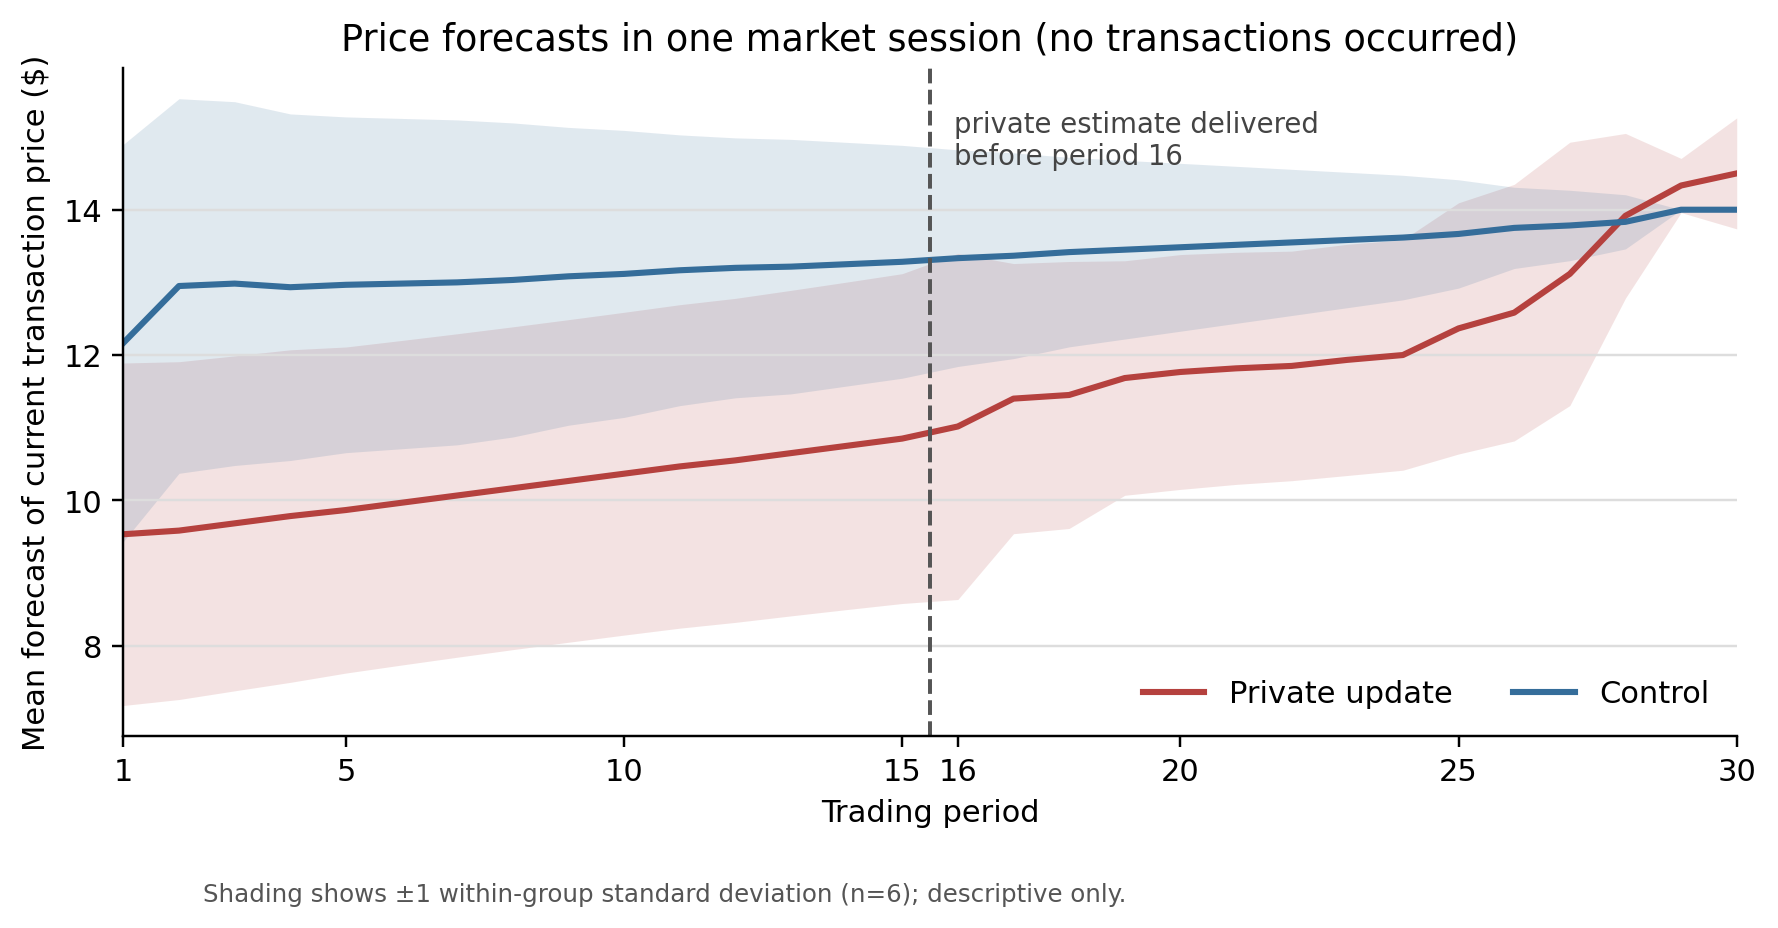
\includegraphics[width=0.9\linewidth]{forecast_paths.png}
\caption{Mean current-price forecast by treatment group. Shading is one
within-group standard deviation ($n=6$ per group); it is descriptive, not an
uncertainty interval. The dashed line marks delivery before period 16. No
transactions occurred in any period.}
\end{figure}

The pilot's main result is market inactivity, not a causal estimate of
information. The information treatment was successfully delivered and
distinguished in private state; it did not create a two-sided market. A useful
next design would give traders varied strategic roles or stronger order-choice
instructions and repeat the treatment over independently seeded markets.

\section{Machine and private view}
EDSL's `call\_market` supplies account, order, public tape, period, settlement,
interest, dividend, and redemption state. This study extends that machine with
one private map and a command that writes an update for one named trader. The
read-only view projects only the current trader's message:

\begin{lstlisting}
machine.fields["private_updates"] = state_field(StateType.map(), {})
machine.commands["publish_update"] = Command(
    inputs={"recipient": StateType.text(), "message": StateType.text()},
    effects=(put("private_updates", arg("recipient"), arg("message")),),
)
machine.view["your_update"] = field("private_updates").get(current("name"))
machine.validate()
\end{lstlisting}

`private\_updates` is not exposed as a whole in `machine.view`. Each trader's
rendered prompt reads `your\_update`; the DSL evaluates that projection using
the current participant name. A missing map entry renders as “No private
analyst update has been issued to you.” Thus the treatment is durable shared
state, while the view enforces participant-specific disclosure.

The machine diagram below was produced by EDSL's `Machine.show\_diagram`
method with the pydot renderer and detailed labels. It shows native market
state and the one map, command, and private projection added for this study.
\begin{figure}[ht]
\centering
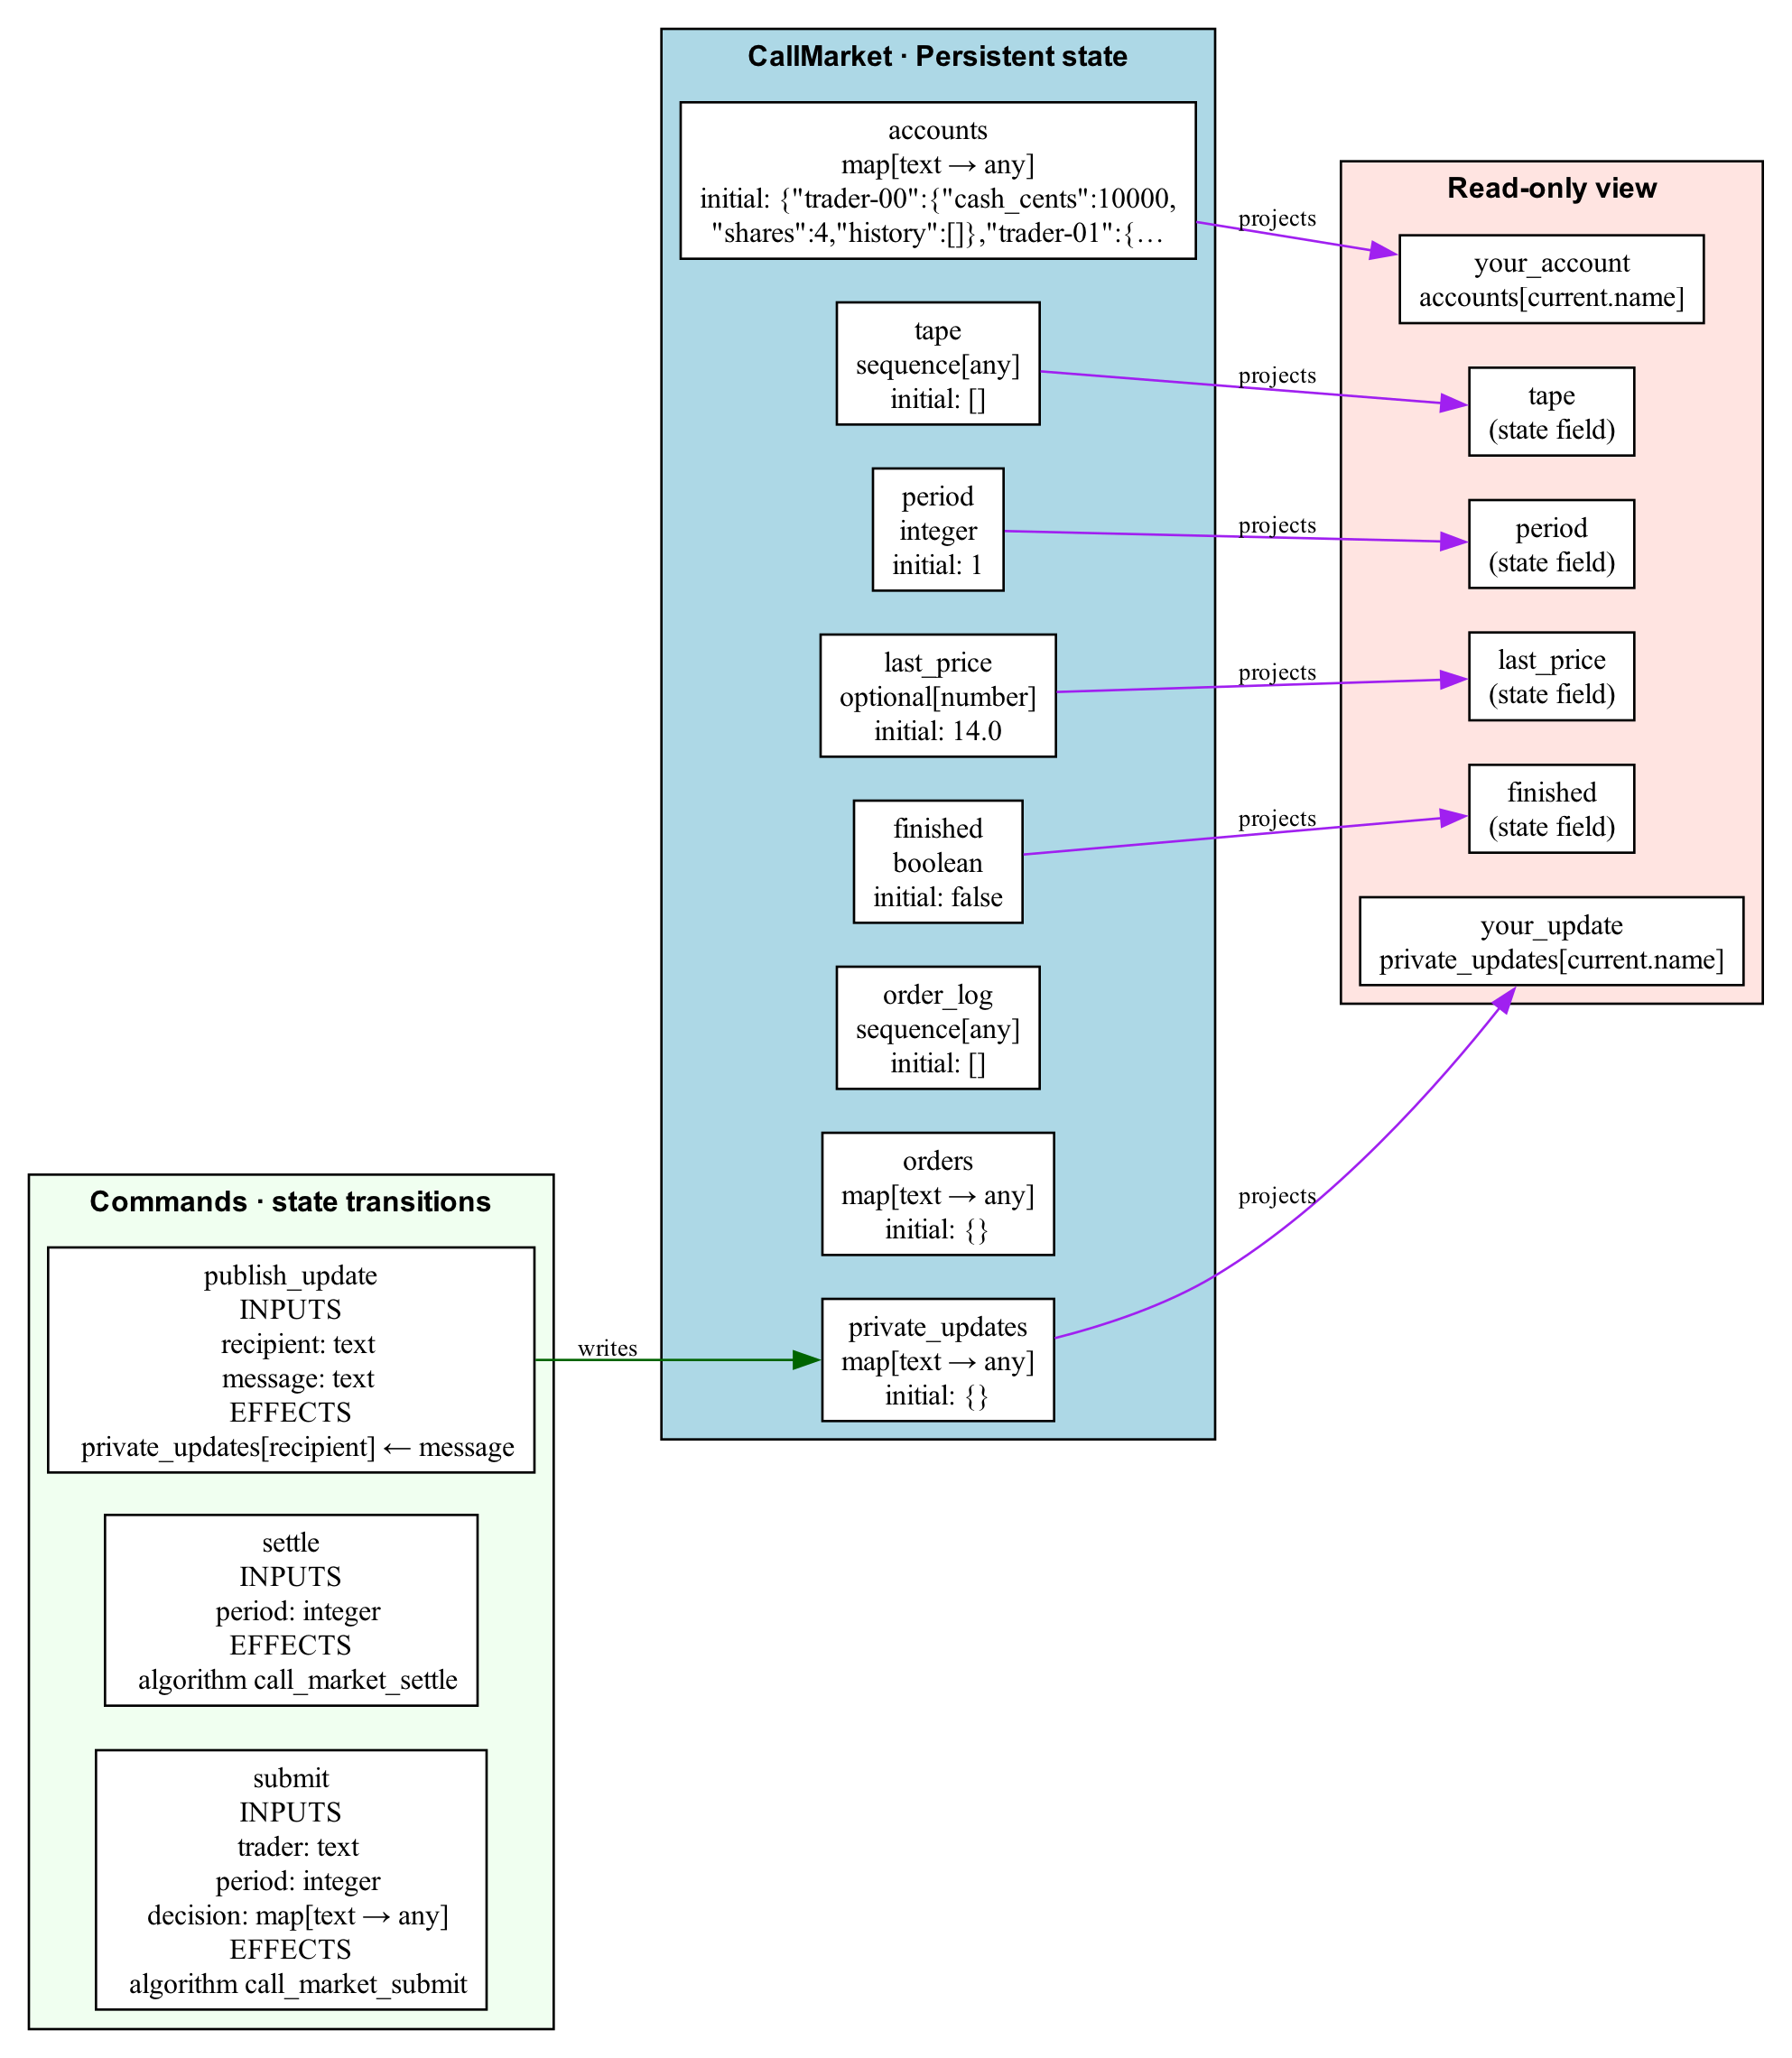
\includegraphics[width=0.68\linewidth,height=0.68\textheight,keepaspectratio]{market_machine.png}
\caption{EDSL-generated state-machine diagram for the extended call market.}
\end{figure}

\clearpage
\section{Workflow: one round and the midpoint transition}
Each period has a trader order step followed by an exchange settlement step.
The order step reads the market and submits each answer as a command. The
settlement step runs the deterministic market algorithm. Immediately after
period 15 settles, six scripted exchange work items write individual update
messages to the private map; period 16 orders depend on those writes. This
ordering ensures the treated traders see the update in period 16 and earlier
rounds cannot see it.

\begin{lstlisting}
orders = workflow.step(
    f"orders-{period}", Survey([decision]),
    assigned_to=role("trader"), after=previous,
    visible_to=role("exchange"), reads=(market.read(),),
    writes=(market.submit(
        trader=current.agent.name, period=period,
        decision=decision.answer,
    ),),
)
settled = workflow.step(
    f"settle-{period}", settlement_survey,
    assigned_to=role("exchange"), after=orders,
    writes=(market.settle(period=period),),
)
previous = settled
if period == 15:
    for recipient in recipients:
        previous = workflow.step(
            f"publish-private-update-{recipient}", update_survey,
            assigned_to=role("exchange"), after=previous,
            writes=(market.publish_update(
                recipient=recipient, message=UPDATE,
            ),),
        )
\end{lstlisting}

The update steps are chained, giving every publication an auditable order in
the workflow event log. The final period's settlement redeems all remaining
shares for \$14 and marks the market finished. All 396 work items completed.

\section{Launch}
The experiment is built from `experiment.py` and run locally through EDSL with
the provider configured in the local environment. Preparation serializes the
specification without making model calls:

\begin{lstlisting}
python3 edsl_replication/studies/asset_market_midpoint_news/experiment.py \
  --output edsl_replication/studies/asset_market_midpoint_news/pilot_01 \
  --prepare-only
\end{lstlisting}

The live pilot used the same command without `--prepare-only`. EDSL's object
store uses its default local application-support directory; job, workflow,
state, and raw response artifacts are also preserved under `pilot\_01/`.

\section{Response recovery and interpretation}
Four final-period responses returned `null` for forecasts beyond the terminal
horizon. Since the decision schema requires numeric forecasts, those responses
were not accepted. The run retained successful responses and state events.
The recovery filled the 12 null out-of-horizon forecast fields with \$14, the
known terminal redemption amount, and then let the ordinary shared-state
workflow settle period 30. The source responses were not overwritten; each
filled participant-field pair is recorded in `recovery.json`. These forecasts
do not determine the final period's order. The prompt now makes the terminal
forecast rule explicit. No additional model calls were required for recovery.

The pilot contains one market, not independent market replications. Traders
share a public tape, so mixed treatment can create interference across traders
when trades occur. Here no trades occurred, so this channel did not activate.
Forecast comparisons and the lone treated buy order should be read as
descriptive evidence about this model, prompt, and session only.

\end{document}
